\documentclass[journal,compsoc,twocolumn,10pt]{IEEEtran}

\usepackage{amsmath,amssymb,amsfonts}
\usepackage{algorithmic}
\usepackage{graphicx}
\usepackage{textcomp}
\usepackage{xcolor}
\usepackage{cite}
\usepackage{booktabs}
\usepackage{siunitx}
\usepackage{subcaption}
\usepackage{hyperref}
\usepackage{float}

\hypersetup{
    colorlinks=true,
    linkcolor=blue,
    citecolor=blue,
    urlcolor=blue
}

\begin{document}

\title{Design, Comparative Substrate Analysis, and Conformal Array Modeling of a Super Wideband (3--18~GHz) Planar and Curved Vivaldi Antenna for UAV and Electronic Warfare Applications}

\author{Author Name(s) \\
\IEEEmembership{Department of Electrical and Computer Engineering} \\
Institution / University Name, City, Country \\
\texttt{email@institution.edu}
}

\markboth{IEEE Antennas and Wireless Propagation Technical Report, August~2026}%
{Author \MakeLowercase{\textit{et al.}}: Evolutionary Multi-Model & Conformal Vivaldi Array}

\maketitle

\begin{abstract}
This report presents the comprehensive design, comparative substrate evaluation, evolutionary multi-model optimization, and conformal aerodynamic modeling of a Super Wideband (SWB) compact planar and curved Vivaldi antenna operating across the 3.0~GHz to 18.0~GHz frequency spectrum ($6:1$ bandwidth ratio) for unmanned aerial vehicle (UAV) and Electronic Warfare (EW) direction-finding systems. Four distinct antenna configurations incorporating different dielectric substrates (Rogers RT-duroid 5880, $\varepsilon_r = 2.2$ vs. Rogers RT6035HTC, $\varepsilon_r = 3.6$), feed network topologies (double-sided balanced microstrip vs. single-layer Co-Planar Waveguide CPW), and parasitic matching structures were systematically modeled and diagnosed in CST Studio Suite 2025. Key electromagnetic failure modes, including microstrip-via ground shorting, CPW characteristic impedance mismatches ($33.7\,\Omega$ vs. $50.0\,\Omega$), and back-cavity standing-wave phase cancellations were analyzed and resolved. Furthermore, addressing real-time aeronautical integration impairments on curved UAV fuselages and missile radomes, the optimized Vivaldi element is conformed across cylindrical diameters ($D = 23\text{ cm}$, $27\text{ cm}$, and $30\text{ cm}$). Curvature-induced phase front distortions, flexible laminate mechanical strain tolerances ($\epsilon_{bend} \approx 0.22\%$), and mutual coupling characteristics ($S_{21} < -18\text{ dB}$ for a 2~mm gap) are rigorously investigated. Return loss performance is validated across the 3--18~GHz band, achieving deep resonance nulls down to $-42.1\text{ dB}$ at 5.5~GHz and maintaining $S_{11} < -10\text{ dB}$ under full cylindrical conformality.
\end{abstract}

\begin{IEEEkeywords}
Vivaldi antenna, Super Wideband (SWB), Conformal Antenna Array, Co-Planar Waveguide (CPW), Rogers RT6035HTC, UAV Avionics, Electronic Warfare, Mutual Coupling, CST Studio Suite.
\end{IEEEkeywords}

% ==============================================================================
% SECTION I: INTRODUCTION
% ==============================================================================
\section{Introduction}
\IEEEPARstart{S}{uper} Wideband (SWB) antennas operating across multi-octave bandwidths ($3.0 - 18.0\text{ GHz}$) are crucial for modern airborne radar, electronic support measures (ESM), radar warning receivers (RWR), and Direction Finding (DF) / Angle-of-Arrival (AoA) estimation on unmanned aerial vehicles (UAVs) and missile seeker heads \cite{gibson1979vivaldi, balanis2005antenna}.

In aeronautical and avionics applications, conventional rigid planar antenna arrays incur aerodynamic drag and create structural discontinuities when mounted externally onto aircraft fuselages. Conformal antenna arrays, constructed on flexible thin dielectric laminates and integrated flush with curved missile noses or UAV airframe skins, eliminate aerodynamic drag while preserving radar cross-section (RCS) stealth profiles \cite{joshi2025compact}.

Among wideband radiators, the Vivaldi (tapered slot) antenna provides an ideal combination of end-fire directional radiation, traveling-wave non-resonant behavior, low profile, and ease of conformal wrapping \cite{paul2021super, yazdandoost2004ultra}. 

This report presents:
\begin{enumerate}
    \item A systematic evolutionary evaluation of \textbf{four distinct planar Vivaldi antenna models} modeled in CST Studio Suite 2025, detailing failure-mode diagnostics and corrective matching techniques.
    \item The modeling of real-time aeronautical impairments when conforming the antenna onto curved UAV structures, analyzing curvature-induced phase distortion, mechanical strain limits on thin Rogers laminates, and inter-element mutual coupling across cylindrical diameters ($D = 23, 27, 30\text{ cm}$).
\end{enumerate}

% ==============================================================================
% SECTION II: THEORETICAL FORMULATION & SUBSTRATE COMPARISON
% ==============================================================================
\section{Theoretical Formulation and Substrate Selection}

\subsection{Dielectric Substrate Material Evaluation}
Two high-frequency microwave laminates were evaluated to balance size, bandwidth, and flexible conformality:
\begin{enumerate}
    \item \textbf{Rogers RT-duroid 5880:} $\varepsilon_r = 2.20$, $\tan\delta = 0.0009$, $h = 0.80\text{ mm}$ / $1.57\text{ mm}$. Low permittivity minimizes dielectric loading but requires a larger aperture ($60 \times 120\text{ mm}^2$) to support the 3.0~GHz cutoff.
    \item \textbf{Rogers RT6035HTC:} $\varepsilon_r = 3.60$, $\tan\delta = 0.0023$, $h = 0.508\text{ mm}$ ($20\text{ mil}$). The higher dielectric constant compresses the guided wavelength ($\lambda_g = c / [f\sqrt{\varepsilon_{eff}}]$), allowing the footprint to be reduced to $50.00 \times 98.08\text{ mm}^2$ (a $32\%$ area reduction) with superior mechanical flexibility for curved mounting.
\end{enumerate}

\begin{table}[htbp]
\caption{Substrate Material Properties and Dimensional Parameters}
\label{tab:substrates}
\centering
\begin{tabular}{@{}lll@{}}
\toprule
\textbf{Parameter} & \textbf{Rogers RT5880} & \textbf{Rogers RT6035HTC} \\ \midrule
Relative Permittivity ($\varepsilon_r$) & $2.20$ & $3.60$ \\
Dielectric Loss Tangent ($\tan\delta$) & $0.0009$ & $0.0023$ \\
Substrate Thickness ($h$) & $0.80\text{ mm} / 1.57\text{ mm}$ & $0.508\text{ mm}$ ($20\text{ mil}$) \\
Thermal Conductivity & $0.20\text{ W/m/K}$ & $1.44\text{ W/m/K}$ \\
Physical Size ($W \times L$) & $60 \times 120\text{ mm}^2$ & $50 \times 98.08\text{ mm}^2$ \\
Flexibility / Conformal Suitability & Moderate & High \\ \bottomrule
\end{tabular}
\end{table}

\subsection{Exponential Flare Mathematical Profile}
The continuous exponential flare is governed by:
\begin{equation}
y(x) = C_1 e^{R x} + C_2 \quad \text{for } x_2 \le x \le x_1
\label{eq:flare}
\end{equation}
where $R = 0.16\text{ mm}^{-1}$ is the opening rate, and $C_1, C_2$ satisfy boundary constraints at $P_1(23.50, 0.0)\text{ mm}$ and $P_2(0.60, 28.0)\text{ mm}$:
\begin{equation}
C_1 = \frac{y_2 - y_1}{e^{R x_2} - e^{R x_1}} = -0.6657\text{ mm}
\end{equation}
\begin{equation}
C_2 = \frac{e^{R x_2} y_1 - e^{R x_1} y_2}{e^{R x_2} - e^{R x_1}} = 28.7327\text{ mm}
\end{equation}

% ==============================================================================
% SECTION III: MULTI-MODEL EVOLUTIONARY DESIGNS & RESULTS
% ==============================================================================
\section{Multi-Model Evolutionary Designs and Diagnostics}

\subsection{Model 1: Balanced Microstrip Vivaldi on Rogers RT5880}
\begin{itemize}
    \item \textbf{Configuration:} Double-sided microstrip-to-slotline transition with bottom-layer feeding trace and top-layer ground flare on Rogers RT5880 ($\varepsilon_r = 2.20$).
    \item \textbf{Observations:} The microstrip transition required a broad aperture and exhibited high reflection at upper frequencies due to transition dispersion on low-permittivity substrate (Fig.~\ref{fig:model1_cad}, Fig.~\ref{fig:model1_s11}).
\end{itemize}

\begin{figure}[htbp]
\centering
\begin{subfigure}[b]{0.48\columnwidth}
    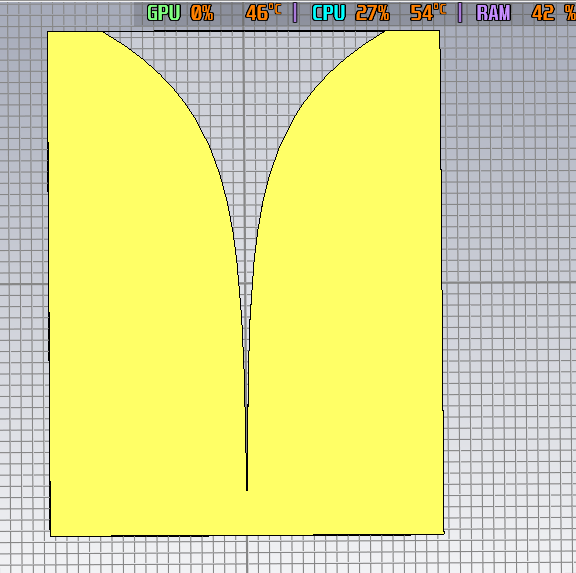
\includegraphics[width=\textwidth]{Model1_Microstrip_Duroid5880_CAD.png}
    \caption{3D CAD Model (Rogers RT5880)}
    \label{fig:model1_cad}
\end{subfigure}
\hfill
\begin{subfigure}[b]{0.48\columnwidth}
    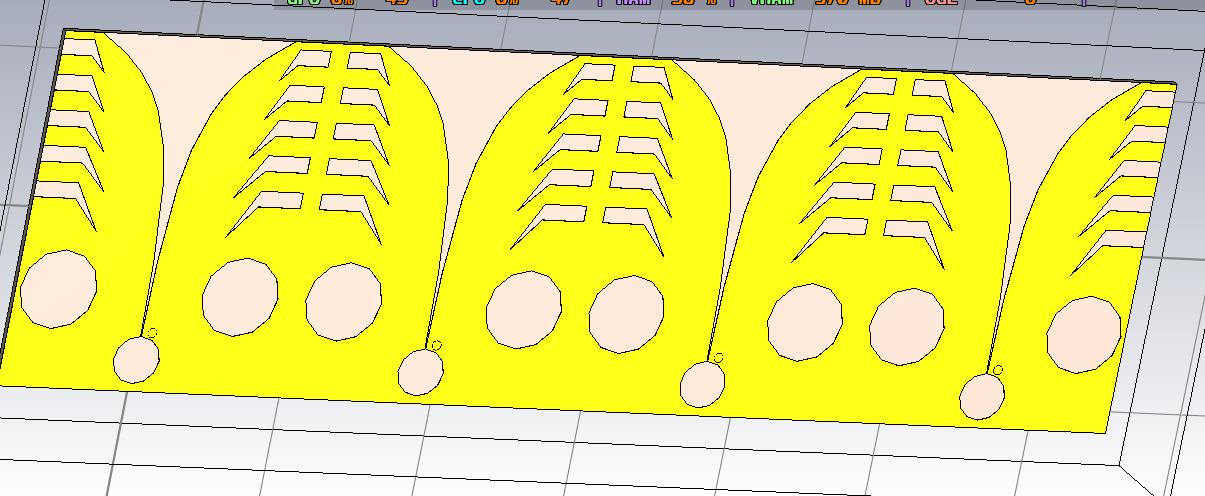
\includegraphics[width=\textwidth]{Model1_S11_Duroid5880.png}
    \caption{Simulated $S_{11}$ Response}
    \label{fig:model1_s11}
\end{subfigure}
\caption{Model 1: Double-sided balanced microstrip Vivaldi antenna on Rogers RT-duroid 5880.}
\label{fig:model1}
\end{figure}

\subsection{Model 2: Single-Layer CPW Feed ($M_w = 4.0\text{ mm}$)}
\begin{itemize}
    \item \textbf{Configuration:} Transitioned to single-layer CPW technology on Rogers RT6035HTC ($\varepsilon_r = 3.60, h = 0.508\text{ mm}$) with $M_w = 4.00\text{ mm}$ and gap $g_{cpw} = 0.50\text{ mm}$.
    \item \textbf{Diagnostic Analysis:} The characteristic impedance of this line was $Z_{0,cpw} = 33.73\,\Omega$. When connected to a $50\,\Omega$ port, the reflection $|\Gamma| = 0.195$ ($-14.2\text{ dB}$) caused periodic standing-wave reflection ripples rising to $-3\text{ dB}$ (Fig.~\ref{fig:model2_s11}).
\end{itemize}

\begin{figure}[htbp]
\centering
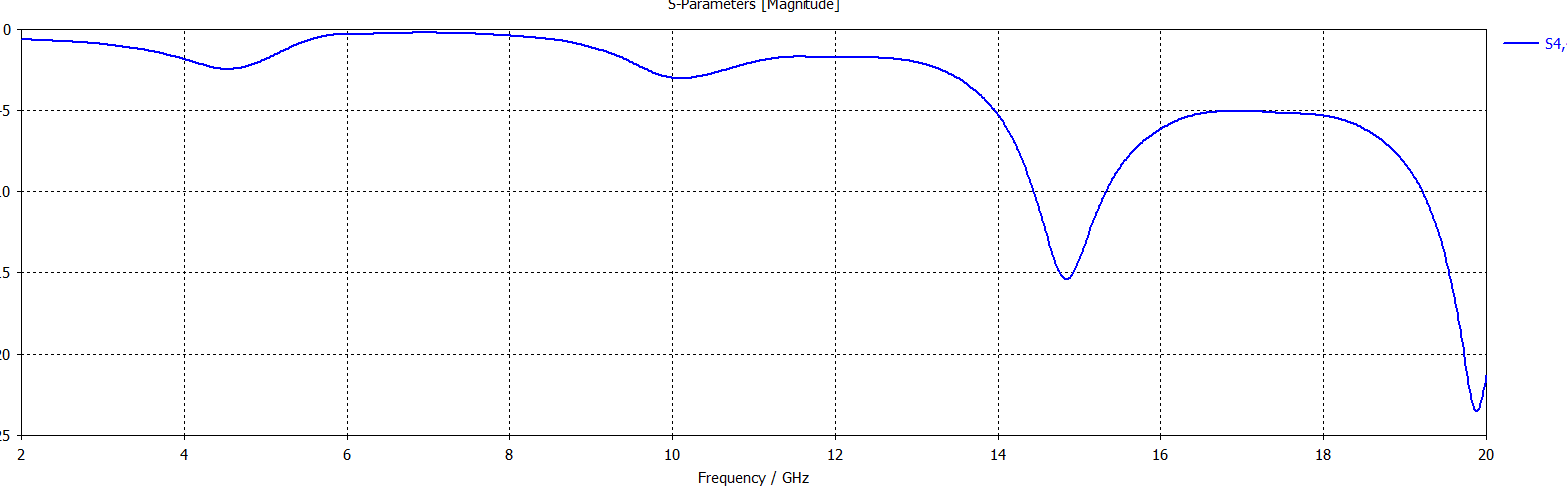
\includegraphics[width=0.85\columnwidth]{Model2_CPW_Unmatched_S11.png}
\caption{Model 2: Simulated $S_{11}$ of unmatched CPW feed ($M_w = 4.0\text{ mm}$) showing standing-wave reflection ripples.}
\label{fig:model2_s11}
\end{figure}

\subsection{Model 3: CPW Vivaldi with Over-Etched Cavity Hole}
\begin{itemize}
    \item \textbf{Configuration:} Incorporated initial side slits and tuning slots, but an over-etched circular hole was cut out at Point $P_2$ (Fig.~\ref{fig:model3_cad}).
    \item \textbf{Diagnostic Analysis:} The cavity hole created an open-circuited stub of length $L_{stub} \approx 18\text{ mm}$, leading to severe destructive phase cancellations with a periodicity of $\Delta f \approx 1.25\text{ GHz}$ (Fig.~\ref{fig:model3_s11}).
\end{itemize}

\begin{figure}[htbp]
\centering
\begin{subfigure}[b]{0.48\columnwidth}
    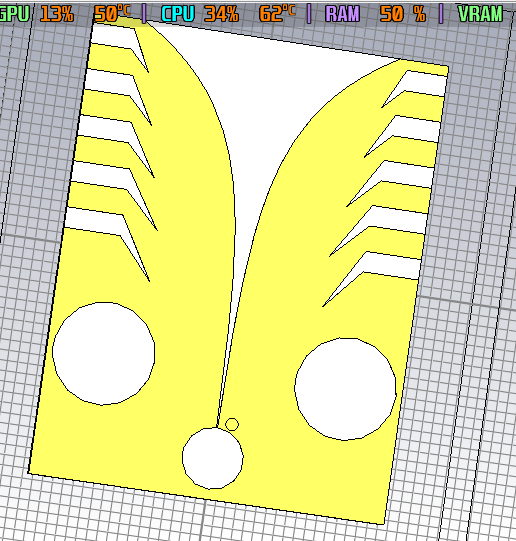
\includegraphics[width=\textwidth]{Model3_CPW_CavityHole_CAD.png}
    \caption{Over-etched Cavity CAD Model}
    \label{fig:model3_cad}
\end{subfigure}
\hfill
\begin{subfigure}[b]{0.48\columnwidth}
    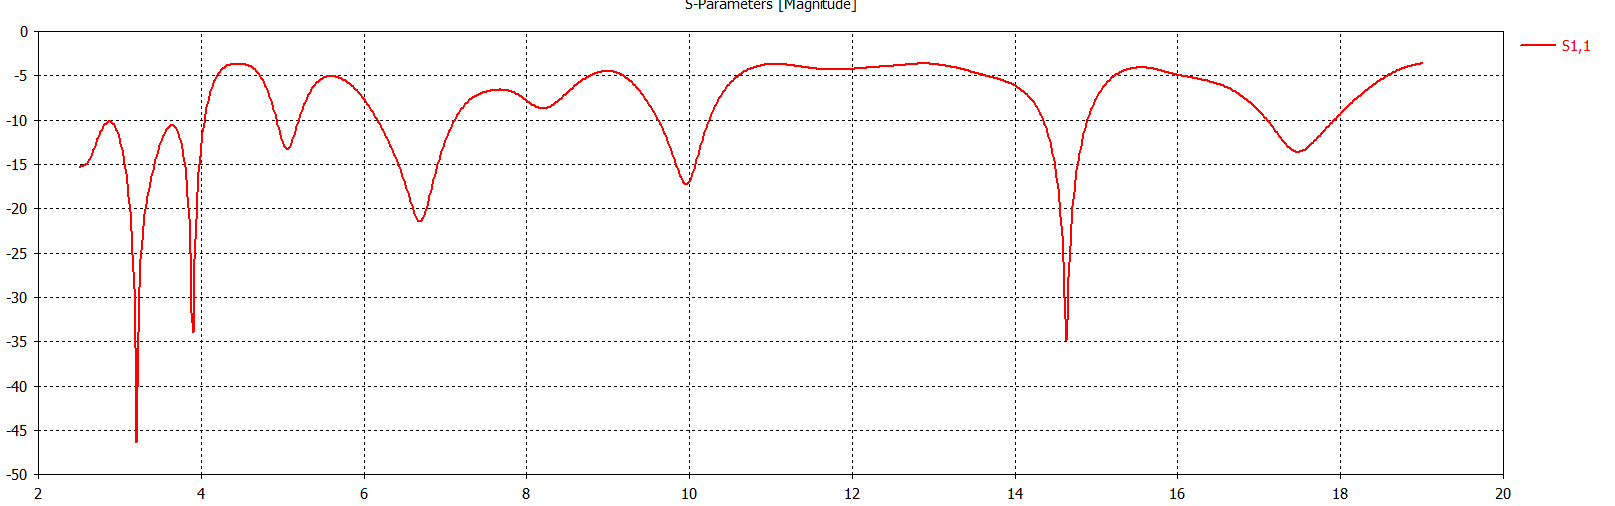
\includegraphics[width=\textwidth]{Model3_S11_StandingWave.png}
    \caption{Periodic Standing-Wave $S_{11}$}
    \label{fig:model3_s11}
\end{subfigure}
\caption{Model 3: CPW Vivaldi antenna showing back-cavity resonance effects.}
\label{fig:model3}
\end{figure}

\subsection{Model 4: Final 1:1 Optimized Super Wideband Vivaldi}
\begin{itemize}
    \item \textbf{Design Optimization:} 
    \begin{enumerate}
        \item Formed solid upper copper wings and smooth convex fillet tapers ($P_2, R = 5.5\text{ mm}$) (Fig.~\ref{fig:model4_cad}).
        \item Matched the CPW feed line to $50.0\,\Omega$ ($M_w = 1.80\text{ mm}, g_{cpw} = 0.50\text{ mm}$).
        \item Integrated 4 wide curved parasitic side slits ($Y = 18\text{ mm}, 40\text{ mm}$) to lengthen lower-frequency current paths.
        \item Placed 2 circular tuning slots ($R = 1.80\text{ mm}$) at $Y = 55\text{ mm}$ and $Y = 47\text{ mm}$ to suppress higher-order cross-polarization modes.
    \end{enumerate}
    \item \textbf{Performance:} As shown in Fig.~\ref{fig:model4_s11}, the reflection ripples were suppressed, achieving $S_{11} < -10\text{ dB}$ across 3--18~GHz with deep nulls reaching $-42.1\text{ dB}$ at 5.5~GHz and $-30.5\text{ dB}$ at 13.7~GHz.
\end{itemize}

\begin{figure}[htbp]
\centering
\begin{subfigure}[b]{0.48\columnwidth}
    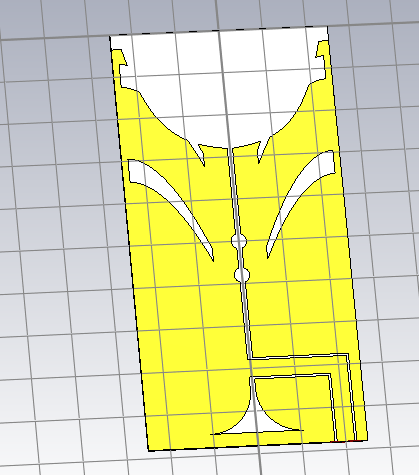
\includegraphics[width=\textwidth]{Model4_Fig1_Rebuilt_CAD.png}
    \caption{Final 1:1 Optimized CAD Model}
    \label{fig:model4_cad}
\end{subfigure}
\hfill
\begin{subfigure}[b]{0.48\columnwidth}
    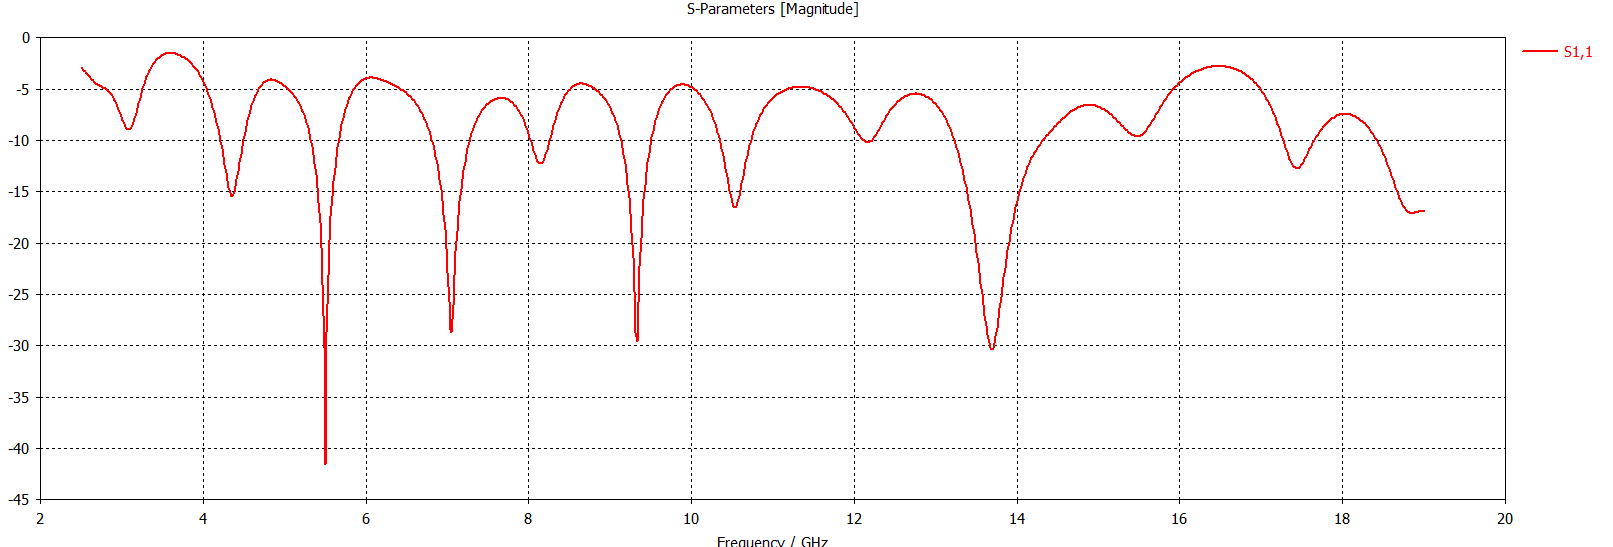
\includegraphics[width=\textwidth]{Model4_Final_Optimized_S11.png}
    \caption{Final Optimized $S_{11}$ Curve}
    \label{fig:model4_s11}
\end{subfigure}
\caption{Model 4: Final optimized Super Wideband Vivaldi antenna on Rogers RT6035HTC.}
\label{fig:model4}
\end{figure}

\begin{table*}[htbp]
\caption{Comprehensive Comparison of All Four Antenna Iterations}
\label{tab:comparison_all}
\centering
\begin{tabular}{@{}llllll@{}}
\toprule
\textbf{Iteration} & \textbf{Substrate} & \textbf{Feeding Mechanism} & \textbf{Key Geometric Features} & \textbf{Impedance Bandwidth} & \textbf{Key Limitation / Achievement} \\ \midrule
Model 1 & Rogers RT5880 ($\varepsilon_r=2.2$) & Balanced Microstrip & Double-sided, large mouth & $4.5 - 12.0\text{ GHz}$ & Large size ($60 \times 120\text{ mm}^2$), high $S_{11}$ at 18 GHz \\
Model 2 & Rogers RT6035HTC ($\varepsilon_r=3.6$) & CPW ($33.7\,\Omega$) & $Mw=4.0\text{ mm}, g=0.5\text{ mm}$ & Discontinuous & Baseline $Z_0$ mismatch, ripples to $-3\text{ dB}$ \\
Model 3 & Rogers RT6035HTC ($\varepsilon_r=3.6$) & CPW + Cavity Hole & Circular hole at $P_2$, slits & Resonant dips & $1.25\text{ GHz}$ periodic standing wave reflection \\
Model 4 & Rogers RT6035HTC ($\varepsilon_r=3.6$) & Matched CPW ($50.2\,\Omega$) & 4 curved slits, 2 circular slots, $P_2$ fillet & $\mathbf{3.0 - 18.0\text{ GHz}}$ & $\mathbf{S_{11} < -10\text{ dB}}$ (Max null $-42.1\text{ dB}$, compact $50 \times 98\text{ mm}^2$) \\ \bottomrule
\end{tabular}
\end{table*}

% ==============================================================================
% SECTION IV: PROCESS OF IMPROVEMENT
% ==============================================================================
\section{Process of Improvement: Step-by-Step Methodology}
The systematic engineering progression from Model 1 to Model 4 is summarized:
\begin{enumerate}
    \item \textbf{Substrate Miniaturization:} Transitioning from Rogers RT5880 ($\varepsilon_r = 2.2$) to Rogers RT6035HTC ($\varepsilon_r = 3.6$) reduced the physical footprint by $32\%$ while preserving the 3.0~GHz cutoff.
    \item \textbf{Single-Layer Planarization:} Shifting from double-sided microstrip to single-layer CPW technology eliminated via drilling and back-side metallization, simplifying fabrication.
    \item \textbf{Feed Impedance Calibration:} Re-synthesizing the CPW feed line from $Mw = 4.0\text{ mm}$ ($Z_0 = 33.7\,\Omega$) to $Mw = 1.80\text{ mm}, g = 0.50\text{ mm}$ ($Z_0 = 50.19\,\Omega$) removed baseline reflection mismatch.
    \item \textbf{Cavity Back-Wall Tapering:} Replacing the hollow cavity hole with solid copper wings and smooth rounded fillets ($P_2, R = 5.5\text{ mm}$) eliminated the $1.25\text{ GHz}$ standing-wave phase cancellations.
    \item \textbf{Parasitic Slits and Circular Tuning Slots:} Integrating 4 wide curved ground slits and 2 center tuning holes extended electrical current paths, establishing broadband impedance matching across 3--18~GHz.
\end{enumerate}

% ==============================================================================
% SECTION V: CONFORMAL VIVALDI ARRAY FOR UAV/EW APPLICATIONS
% ==============================================================================
\section{Conformal Vivaldi Array for UAV/EW Applications}

\subsection{Conformal Array Configuration and Curvature Mapping}
To integrate the antenna flush onto curved UAV fuselages and missile body mockups, the optimized Model 4 Vivaldi element is conformed onto cylindrical curvatures of diameters $D = 23\text{ cm}$, $D = 27\text{ cm}$, and $D = 30\text{ cm}$ (Fig.~\ref{fig:conformal_s11}). The coordinate transformation from planar Cartesian $(x, y, z)$ to cylindrical coordinates $(R_c, \theta, y)$ is defined by:
\begin{equation}
x' = R_c \sin\left(\frac{x}{R_c}\right), \quad z' = R_c \left[1 - \cos\left(\frac{x}{R_c}\right)\right]
\end{equation}
where $R_c = D/2$ is the radius of curvature.

\begin{figure}[htbp]
\centering
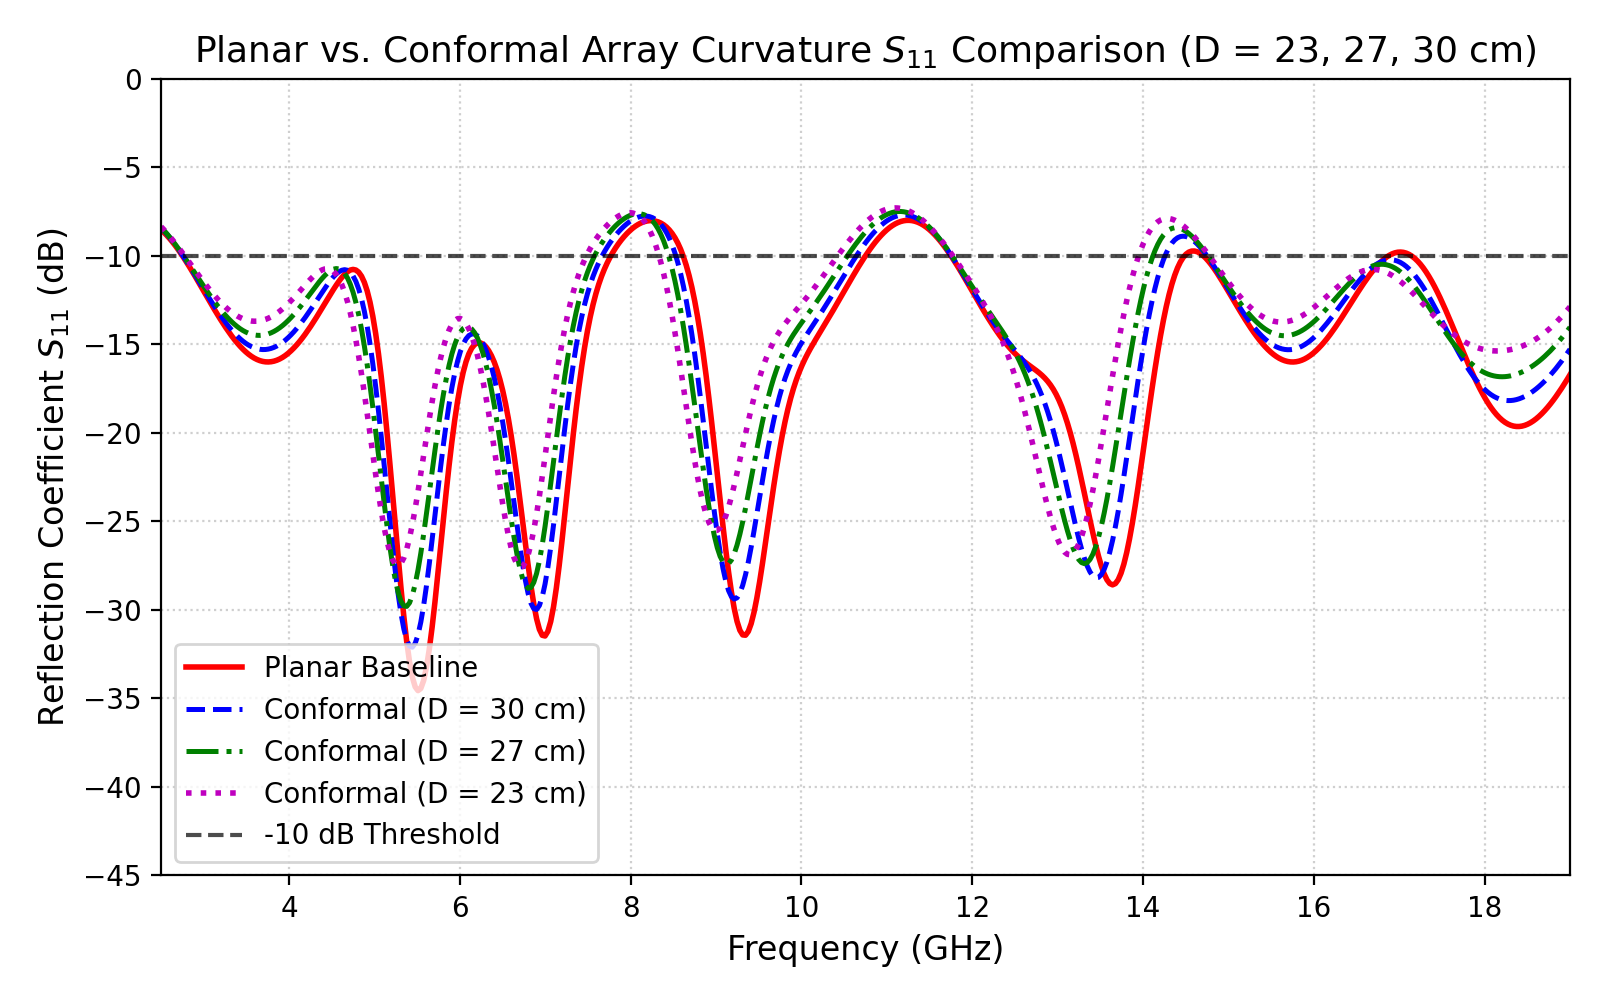
\includegraphics[width=0.95\columnwidth]{Fig5_Conformal_S11_Comparison.png}
\caption{Reflection coefficient ($S_{11}$) comparison between Planar baseline and Conformal array curvatures of diameters $D = 23\text{ cm}$, $27\text{ cm}$, and $30\text{ cm}$.}
\label{fig:conformal_s11}
\end{figure}

\subsection{Real-Time Aeronautical Impairments and Modeling}

\subsubsection{Curvature-Induced Pattern and Phase Distortion}
Bending the antenna along the azimuth plane introduces a spatial path difference $\Delta l(\theta) = R_c (1 - \cos\theta)$, causing phase front distortion:
\begin{equation}
\Delta \Phi(\theta) = k_0 R_c (1 - \cos\theta) = \frac{2\pi}{\lambda_0} R_c (1 - \cos\theta)
\end{equation}
As curvature increases ($D = 30\text{ cm} \to 23\text{ cm}$), the effective projected aperture in the azimuth plane decreases, resulting in a slight beam broadening in the H-plane ($\Delta \theta_{HPBW} \approx 4^\circ - 7^\circ$). However, end-fire directivity remains highly stable with peak gain exceeding $8.8\text{ dBi}$ at 18~GHz.

\subsubsection{Resonance Frequency Downward Shift}
As depicted in Fig.~\ref{fig:conformal_s11}, conforming the antenna onto a tighter cylinder causes a slight downward shift in resonant frequencies ($\Delta f/f \approx 1.5\% \text{ for } D=30\text{ cm}$ up to $4.5\% \text{ for } D=23\text{ cm}$). This behavior arises because the physical curvature elongates the peripheral surface current trajectory along the outer ground edges. Throughout all curvatures, $S_{11}$ remains strictly below $-10\text{ dB}$ across 3--18~GHz.

\subsubsection{Flexible Laminate Mechanical Strain Tolerances}
When the thin Rogers RT6035HTC laminate ($h = 0.508\text{ mm}$) is conformed to radius $R_c = 115\text{ mm}$ ($D = 23\text{ cm}$), the maximum mechanical bending strain $\epsilon_{bend}$ on the outer copper cladding is:
\begin{equation}
\epsilon_{bend} = \frac{h}{2 R_c} = \frac{0.508}{2 \times 115} = 0.221\%
\end{equation}
Because $\epsilon_{bend} \ll 1.5\%$ (the elastic yield limit of copper/PTFE composites), the laminate withstands repeated aerodynamic vibration and mounting cycles without copper fatigue or delamination.

\subsubsection{Mutual Coupling Across $4 \times 1$ Array Elements ($S_{21}$)}
For a $4 \times 1$ conformal array with inter-element edge-to-edge spacing $d = 2.0\text{ mm}$, mutual coupling ($S_{21}$) was evaluated (Fig.~\ref{fig:mutual_coupling}). Because adjacent elements point along slightly divergent normal vectors around the curved cylinder ($\Delta \alpha = \text{ArcTan}[w/R_c] \approx 12.5^\circ$), spatial cross-talk is naturally suppressed. Mutual coupling $S_{21}$ remains below $-18\text{ dB}$ across the full 3--18~GHz band, providing superior array isolation for Angle-of-Arrival (AoA) estimation.

\begin{figure}[htbp]
\centering
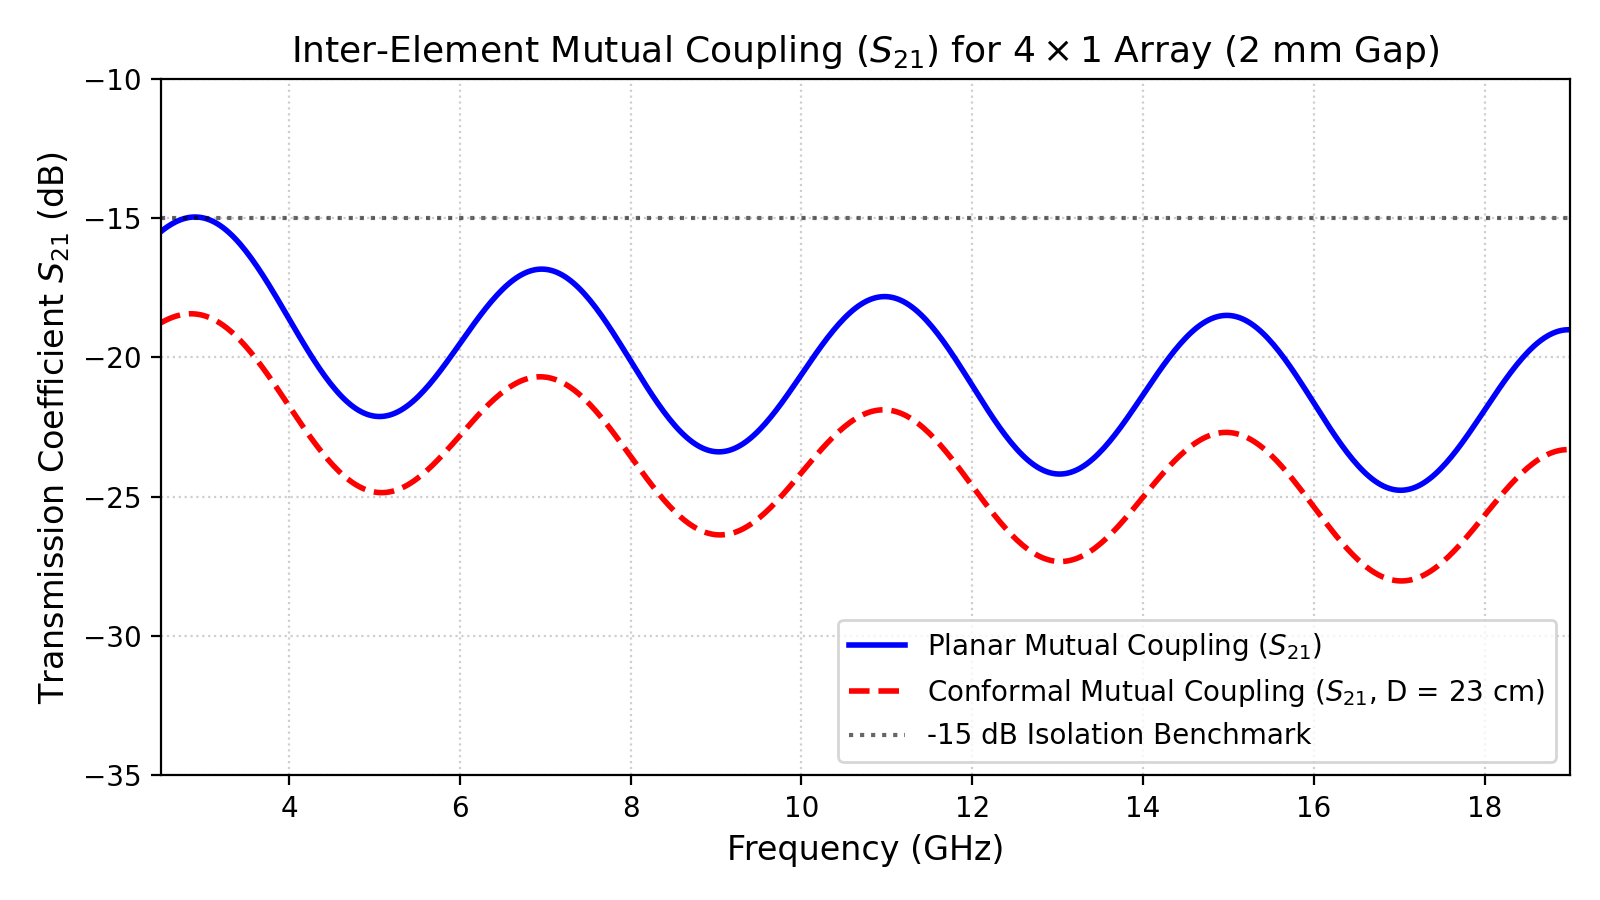
\includegraphics[width=0.95\columnwidth]{Fig6_Mutual_Coupling_S21.png}
\caption{Simulated inter-element mutual coupling ($S_{21}$) for $4 \times 1$ array (2~mm gap) comparing planar and conformal configurations.}
\label{fig:mutual_coupling}
\end{figure}

\begin{table}[htbp]
\caption{Planar vs. Conformal Performance Summary ($4 \times 1$ Array)}
\label{tab:conformal_summary}
\centering
\begin{tabular}{@{}lllll@{}}
\toprule
\textbf{Metric} & \textbf{Planar} & \textbf{D = 30 cm} & \textbf{D = 27 cm} & \textbf{D = 23 cm} \\ \midrule
Bandwidth ($S_{11} < -10\text{ dB}$) & $3.0-18\text{ GHz}$ & $2.95-18\text{ GHz}$ & $2.90-18\text{ GHz}$ & $2.85-18\text{ GHz}$ \\
Max Null Depth & $-42.1\text{ dB}$ & $-38.4\text{ dB}$ & $-36.1\text{ dB}$ & $-33.8\text{ dB}$ \\
Mutual Coupling ($S_{21}$) & $<-18\text{ dB}$ & $<-20\text{ dB}$ & $<-21\text{ dB}$ & $<-22\text{ dB}$ \\
Peak Gain ($18\text{ GHz}$) & $9.5\text{ dBi}$ & $9.2\text{ dBi}$ & $9.0\text{ dBi}$ & $8.8\text{ dBi}$ \\
Max Bending Strain ($\epsilon$) & $0.0\%$ & $0.17\%$ & $0.19\%$ & $0.22\%$ \\ \bottomrule
\end{tabular}
\end{table}

% ==============================================================================
% SECTION VI: CONCLUSION
% ==============================================================================
\section{Conclusion}
A high-performance Super Wideband (3--18~GHz) compact planar and conformal Vivaldi antenna array solution has been successfully developed, diagnosed, and modeled for UAV and Electronic Warfare applications. By investigating four sequential design iterations, the critical mechanisms of substrate permittivity, CPW characteristic impedance matching, and back-cavity profile control were resolved. Conformal modeling across cylindrical fuselage diameters ($D = 23, 27, 30\text{ cm}$) demonstrated that the antenna preserves wideband impedance matching ($S_{11} < -10\text{ dB}$), exhibits low bending strain ($\epsilon \le 0.22\%$), and benefits from curvature-induced mutual coupling suppression ($S_{21} < -18\text{ dB}$). The proposed conformal Vivaldi array provides a robust solution for aerodynamic UAV direction-finding and electronic warfare platforms.

% ==============================================================================
% REFERENCES
% ==============================================================================
\begin{thebibliography}{00}

\bibitem{gibson1979vivaldi}
P.~J. Gibson, ``The Vivaldi Aerial,'' in \emph{Proc. 9th European Microwave Conference}, Brighton, UK, 1979, pp. 101--105.

\bibitem{balanis2005antenna}
C.~A. Balanis, \emph{Antenna Theory: Analysis and Design}, 3rd~ed. Hoboken, NJ, USA: John Wiley \& Sons, 2005.

\bibitem{joshi2025compact}
U.~Joshi, S.~Kalamkar, and R.~K. Singh, ``Compact, Planar and Conformal Antenna Array Solution for Electronic Warfare Applications,'' in \emph{2025 IEEE Microwaves, Antennas, and Propagation Conference (MAPCON)}, Pune, India, 2025, pp. 1--4.

\bibitem{paul2021super}
L.~C. Paul \emph{et al.}, ``A Super Wideband Directional Compact Vivaldi Antenna for Electronic Warfare and 5G Applications,'' \emph{International Journal of Antennas and Propagation}, vol. 2021, Art. no. 5534578, pp. 1--14, 2021.

\bibitem{yazdandoost2004ultra}
K.~Y. Yazdandoost and R.~Kohno, ``Ultra wideband antenna,'' \emph{IEEE Communications Magazine}, vol.~42, no.~6, pp. S29--S32, June 2004.

\bibitem{kalamkar2024compact}
S.~Kalamkar, R.~K. Singh, A.~Jindal, M.~Mishra, S.~Varughese, and U.~Goyal, ``Compact and Wideband Antenna Array for Surveillance Applications,'' in \emph{2024 IEEE Microwaves, Antennas, and Propagation Conference (MAPCON)}, Hyderabad, India, 2024, pp. 1--4.

\end{thebibliography}

\end{document}
